% -----------------------------------------------------------------------------
%      _ _                        _
%   __| (_)___  ___ _   _ ___ ___(_) ___  _ __
%  / _` | / __|/ __| | | / __/ __| |/ _ \| '_ \
% | (_| | \__ \ (__| |_| \__ \__ \ | (_) | | | |
%  \__,_|_|___/\___|\__,_|___/___/_|\___/|_| |_|
% -----------------------------------------------------------------------------
%*?     wc: 1234
%**     wc: 3000
%*[ ]   Draft design patterns
% -----------------------------------------------------------------------------
\chapter{Discussion}
\label{sec: discussion}
\markboth{}{Discussion}
\epigraph{\emph{Alice has stepped through the looking glass [...] It is the job all future artists and activists to use this technology for the better, to bring people together, and uproot social injustice.}}{\citep[]{skwarek2018}}
% -----------------------------------------------------------------------------
\section{From Interface to Instrument} \label{sec: discussion-review}
 Before examining and contextualising the results of \nameref{sec: area}, \nameref{sec: polaris}, and \nameref{sec: polygons}, let us first rendezvous with the initial perspectives on AR that were outlined in \autoref{sec: literature}.

The present thesis began with an exploration of the landscape of historical and contemporary AR research and development. 



% -----------------------------------------------------------------------------
\section{Engaging in a DIY Approach to AR} \label{sec: discussion-method}
\subsection{Approach to Practice / Theory}
\subsection{Outline of Method}
\subsection{Limitations}
\subsection{Proto-Design Pattern}
\subsection{Studies}



% -----------------------------------------------------------------------------
\section{Design Patterns for AR Art and Music} \label{sec: discussion-patterns}
The term design pattern here, is borrowed from the field of computer science, where it is taken to describe ``communicating objects and classes that are customized to solve a general design problem in a particular context'' \citep{gamma1995}. A design pattern thus ``names, abstracts, and identifies the key aspects of a common design structure that make it useful for creating a reusable object-oriented design''. So, while as a method it may not operate completely as it would in its native computer science, to address the outstanding aims of the thesis, design patterns do serve to be less rigid than frameworks, more problem-focused than guidelines; whilst inheriting the meaningful organisational structure that comes with an object-oriented design approach\footnote{explain OOD}. Design patterns are characterised by having four elements:
\begin{itemize}
    %*[ ]   first two look similar
    \item The \textbf{pattern name} describes the design problem at a higher level of abstraction
    \item The \textbf{problem} describes the situation in which you might apply the pattern
    \item The \textbf{solution} describes the relationships between elements of the pattern that aim to solve the problem
    \item The \textbf{consequences} are the results and trade-offs of applying the pattern
\end{itemize}

\begin{figure}
    \centering
    {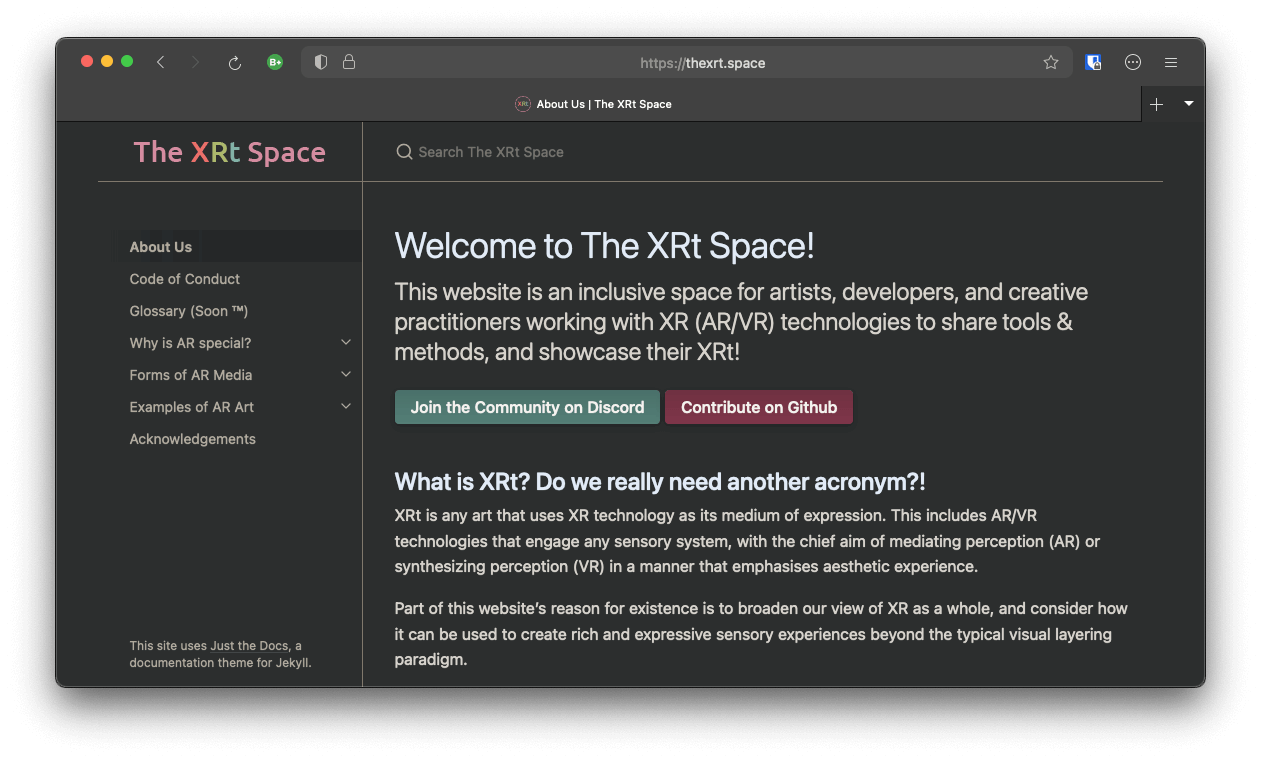
\includegraphics[width=.75\linewidth]{04-method/xrtspace.png}}
    \caption[The XRt Space website]{The XRt Space website}
\end{figure}\label{fig: thexrtspace}

%*[ ]   maybe change xrt.space to github.io link
These design patterns are therefore subject to iteration, and the latest version can be found on \href{https://www.thexrt.space}{the XRt Space website}, a community-editable repository created to host and update them. The principles used to guide the patterns draw on the resistances outlined in \autoref{sec: method-resistance}, namely taking a DIY approach, decoupling from the ocularcentric and layering paradigms of typical AR experience, and attempting to navigate an inherently consumerist space whilst trying not to contribute to exploitative systems of oppression that uphold it. They are also guided by the theoretical proposals of \autoref{sec: theory}: that participant's and performer's cognitive processes in the experience of AR artworks are embodied, embedded, enacted, and extended, and have the potential to be modulated to extents that offer novel aesthetic experiences of augmented \hyperref[sec: theory-materiality]{materiality}, \hyperref[sec: theory-embodiment]{embodiment}, and \hyperref[sec: theory-space]{space}. The following sections outline three design patterns, \textit{\nameref*{sec: discussion-patterns-experience}}, \textit{\nameref*{sec: discussion-patterns-instrument}}, and \textit{\nameref*{sec: discussion-patterns-environment}}.

\subsection{Designing for Rich AR Experience} \label{sec: discussion-patterns-experience} 
\autoref{sec: theory} drew on a number of theoretical propositions, and put forward that AR has the potential to scaffold new modes of performance and expression in the arts and music, furthermore, that from an enactivist approach experience, this would consist in radically modulating the material, embodied, and spatial experience of participants. This is the starting point for ideating and designing an artistic AR experience in the present thesis. This pattern addresses the issue of the typicality of AR experience being simple interactions with visual overlay devices. It approaches experience ideation from a holistic and multisensory, or ``modalities-encompassing'' \citep{schraffenberger2018} perspective. Furthermore, the `4Es' of an enactivist approach can be considered as conditions for what could be described as immersive and ``rich experience" \citep{bilbow2021}. As highlighted in \autoref{sec: theory-materiality-complexitymusic}, enactivist principles have been offered as guidelines for the creation of interactive systems in the past; Essl and O'Modhrain \citeyearpar{essl2006}, Armstrong \citeyearpar{armstrong2006}, and Hayes \citeyearpar{hayes2019} suggest this approach in the design of new musical instruments. 

The concept of rich experience also stands in stark contrast to the current direction of corporate XR technologies, where it is being developed to \textbf{replace} in-person interactions e.g. by facilitating in-headset `work from home' virtual environments such as Meta Horizons. It also stands in contrast with the marketed push towards AR as a tool for driving commerce through targeted advertisements. How as artists and musicians can we avoid the corporate, commercial, ocularcentric, and overlay approach to AR? How can we offset the dystopian hell-scape, painted by designer and film-maker Keiichi Matusda in various film shorts (see \autoref{fig: discussion-matsuda}).

\begin{figure}
    \centering
    \subcaptionbox{\textit{"The Pusher / The Entertainment"} \citeyearpar{matsuda2009}}[.4\linewidth]{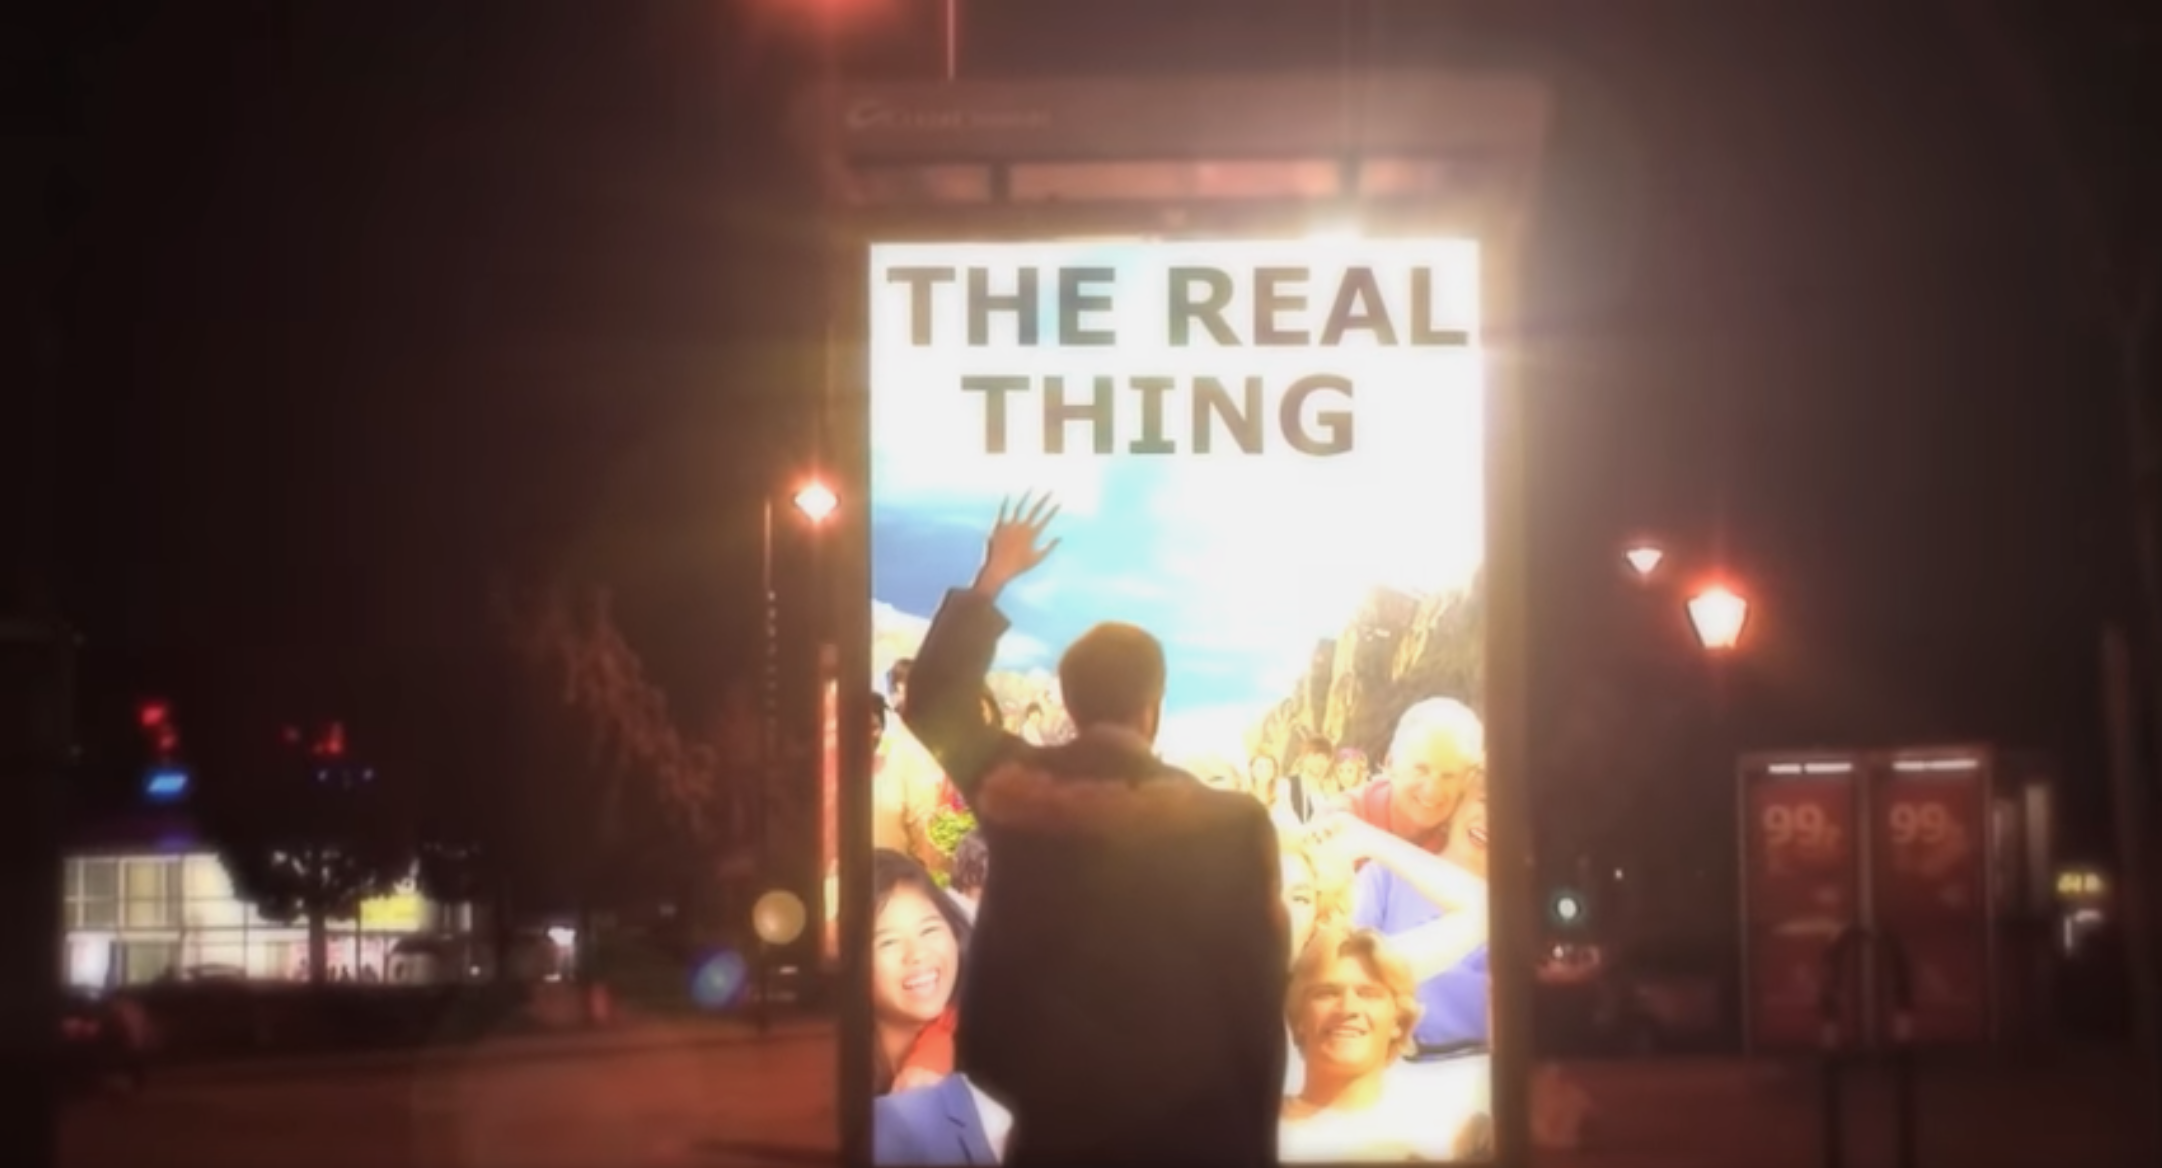
\includegraphics[height=2.5cm]{08-discussion/matsuda2009.png}}
    \subcaptionbox{\textit{"Augmented (hyper)Reality: Domestic Robocop"} \citeyearpar{matsuda2010}}[.4\linewidth]{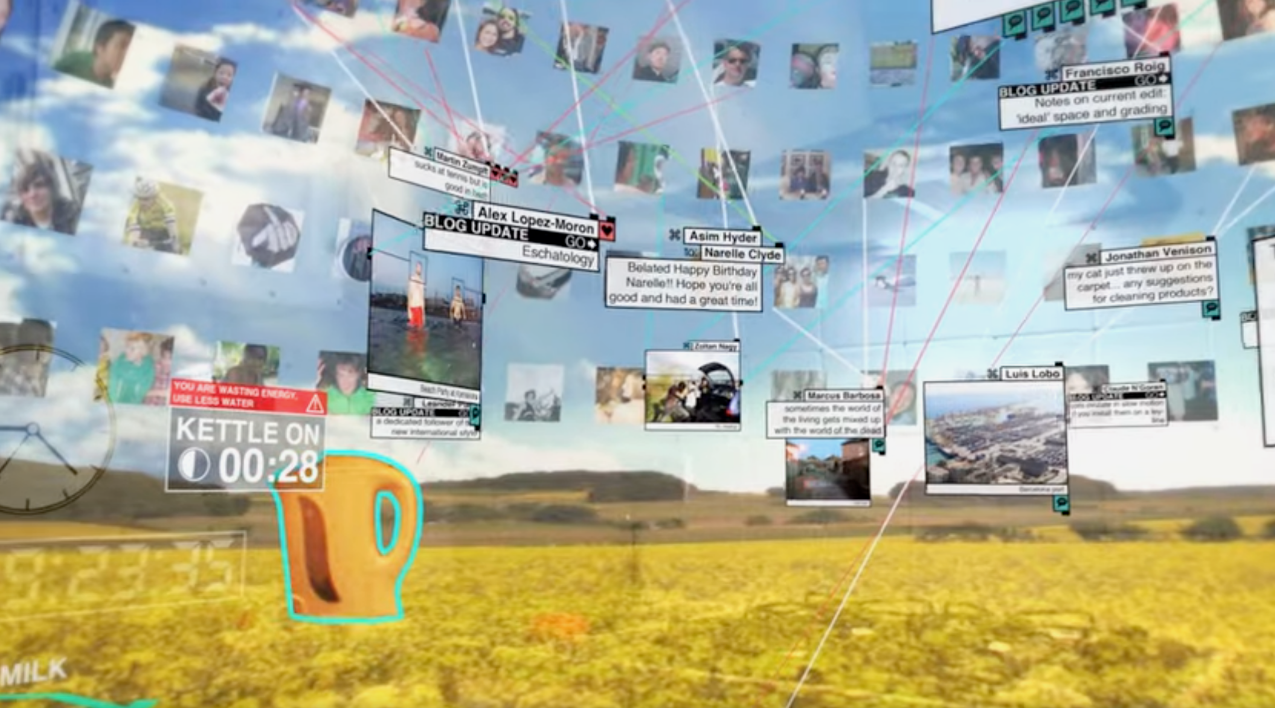
\includegraphics[height=2.5cm]{08-discussion/matsuda2010.png}} \\
    \vspace{0.5cm}
    \subcaptionbox{\textit{"HYPER-REALITY"} \citeyearpar{matsuda2016}}[.4\linewidth]{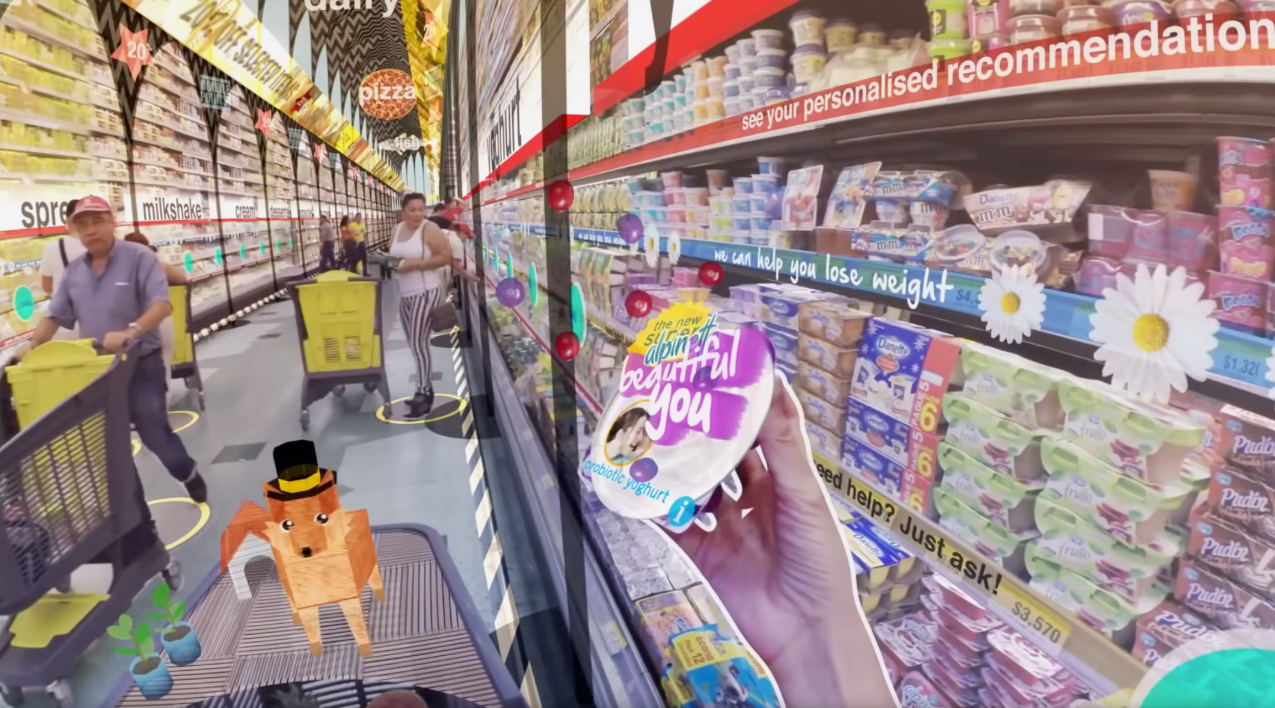
\includegraphics[height=2.5cm]{08-discussion/matsuda2016.png}}
    \subcaptionbox{\textit{"Merger"} \citeyearpar{matsuda2019}}[.4\linewidth]{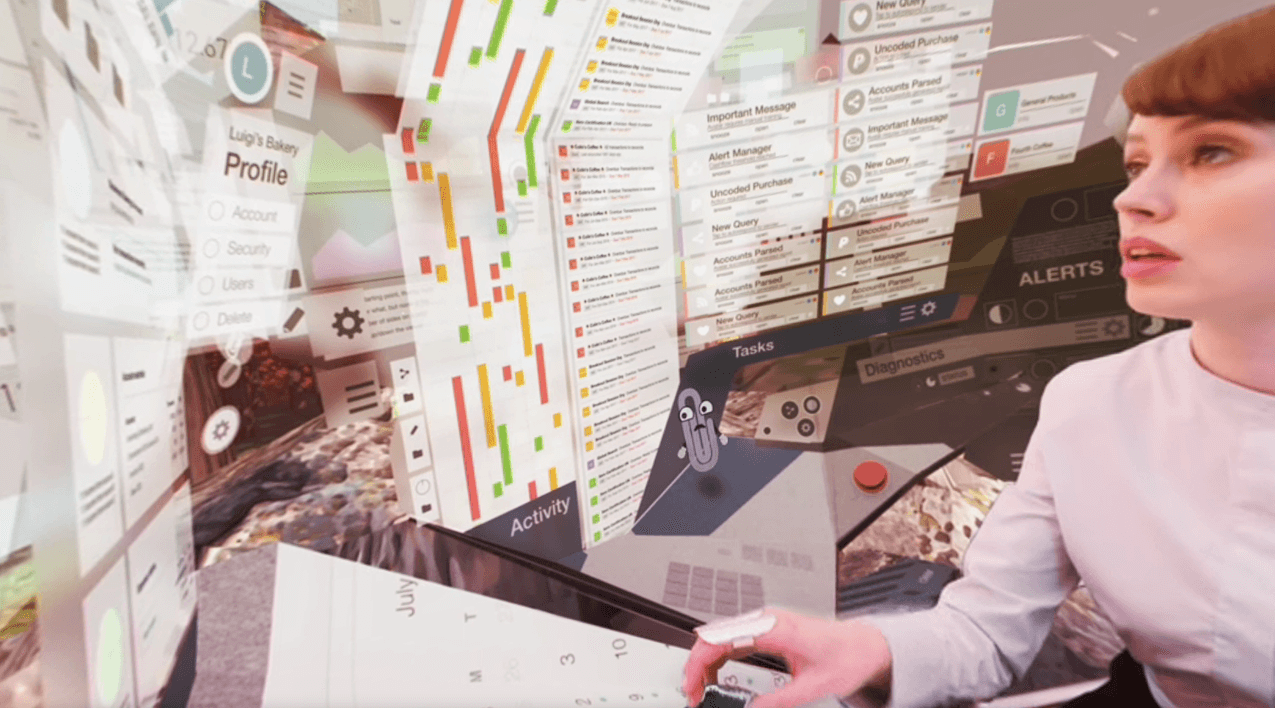
\includegraphics[height=2.5cm]{08-discussion/matsuda2019.png}}
    \caption{Keiichi Matusda's Short Films on AR}
    \label{fig: discussion-matsuda}
\end{figure}

\subsubsection{Centre the experience on two or more sensory interactions}
Whether it is Dewey's concept of the ``live creature'', or the contemporary enactivist's framing of the importance of embodiment, the AR experience ought to be \textit{centred on two or more sensory interactions}. It may include any combination of sensory interaction types, i.e visual (vision), auditory (hearing), vestibular (movement and balance), olfactory (smell), gustatory (taste), and somatosensory (touch). %*! add

\subsubsection{Invoke a meaningful relationship between the real and virtual}
AR's medium specificity, discussed in \autoref{sec: theory-materiality-mediumspec}, should be at the forefront of intentional design choices. If AR is unique because its ``invocation of relationships between real and virtual processes in the axes of spatial, thematic, material and ecological distance'', these relationships become a key handle by which artists and musicians can \textit{meaningfully steer experience to achieve aesthetic experiences}. Consider the following:
\begin{itemize}
    \item Spatial \\
    \item Thematic \\
    \item Material \\
    \item Ecological \\
\end{itemize}

\subsubsection{Implement an AR subform from an enactivist perspective}

\subsubsection{Delineate clear spatial and conceptual boundaries for the participant}
Snippets describe a small-scale clip-like \footnote{Similar in scale to the video-clip, sound-clip, clipart, and now app-clip, however conceptually different in that Snippets are not a miniaturised `extracts' or `segments' of a larger experience} AR Experiences that occur in the approximate interaction space of 30cm3, e.g. between a users hands. The Snippet itself does not supply a full sensorial experience, instead providing two human- to-sense interactions through its AR subforms. Rather than being a fully interactive relationship between real and virtual objects / environments (Behavioural Relationship), Snippets contain simpler, and more reactive Content-based Relationships or Spatial Relationships.

Scenes describe medium-scale AR Experiences that occur on and around the body, an approximate interaction space of 200cm3. They can be formed from existing Snippets, or created from scratch. They ideally feature more (and higher complexity) human-to-sense interactions, and therefore potentially more interactive, Content-based and Spatial Relationships between real and virtual elements will be formed.

Spaces describe large-scale AR Experiences, involving multiple human actors in a variety of differently sized interaction spaces in a room. For example, augmented hand / body interaction with the environment and other users, and multiple of zones of interaction in different sections of the room. Spaces provide fully multisensory immersive experiences, by making use of a combination of different sensory modalities, AR subforms, and Behavioural Relationships.


%*[ ]   Replace with LaTeX table 
%*[ ]   Handles / 4EC
% \begin{figure}
%     \centering
%     {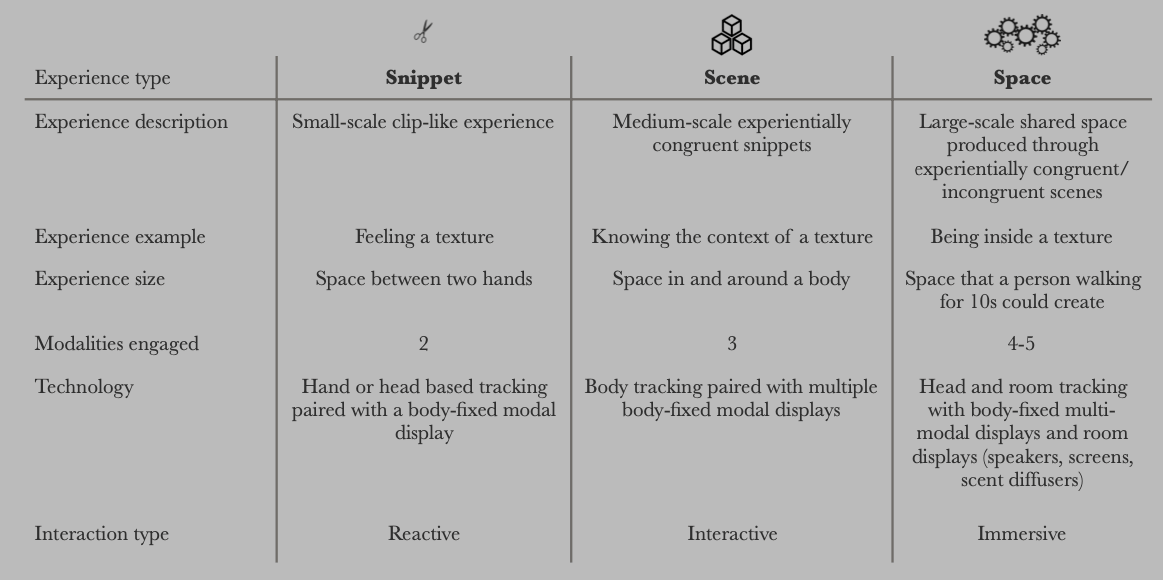
\includegraphics[width=.75\linewidth]{04-method/snippetscenespace.png}}
%     \caption[A Categorisation of AR Interaction Types]{A Categorisation of AR Interaction Types}
% \end{figure}\label{fig: ARinteraction}

\subsection{Consideration of the AR Instrument} \label{sec: discussion-patterns-instrument}
%*[ ]   probably explain the whole experience/piece participant/performer in intro
When describing the means through which a participant or performer meaningfully interacts or engages in any kind of information transfer in the AR system, it is through the AR Instrument. 
%*[ ]   Replace with LaTeX table
\begin{figure}
    \centering
    {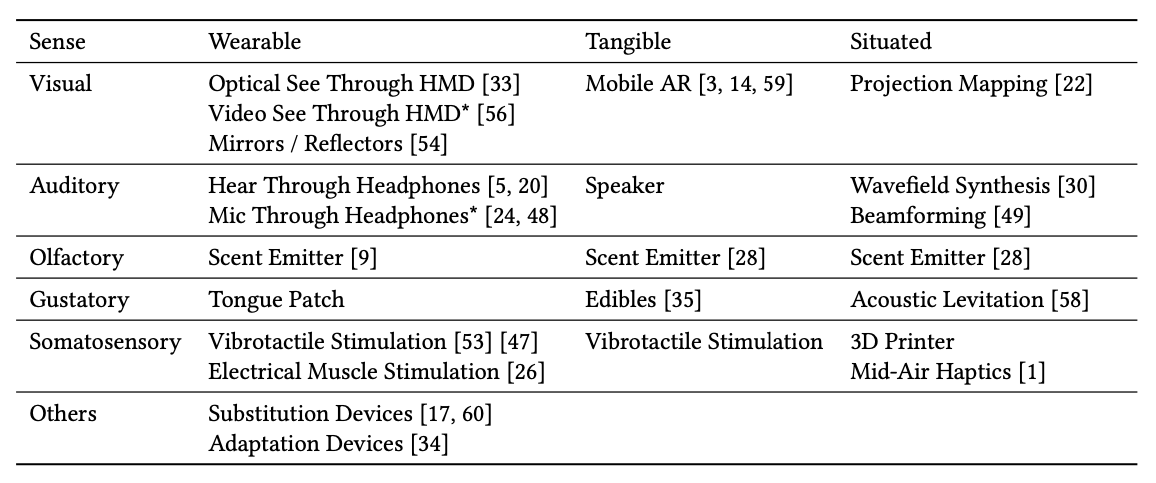
\includegraphics[width=.75\linewidth]{04-method/sensorydisplays.png}}
    \caption[Potential AR Instruments]{Potential AR Instruments}
\end{figure}\label{fig: ARinstrument}
% \begin{table*}
    %     \caption{A classification of potential sensory displays for MSAR Instruments}
    %     \begin{tabular}{lllll}
        %         Sense&Wearable&Tangible&Situated&\\
%         Visual&Optical See Through HMD \tablefootnote{ hi hi\cite{leapmotion2018}}&Mobile AR \tablefootnote{\cite{apple2020,google2020,vuforia2020}}&Projection Mapping \tablefootnote{\cite{lightform2020}} &\\ &Video See Through HMD* \tablefootnote{\cite{varjo2019}}&&&\\ &Mirrors / Reflectors \tablefootnote{\cite{tonn2020}}&&&\\
%         Auditory&Hear Through Headphones \tablefootnote{\cite{kiefer2018,barde2020}}&Speaker&Wavefield Synthesis \tablefootnote{\cite{melchior2005}}&\\&Mic Through Headphones* \tablefootnote{\cite{lindeman2008,sennheiser2018}}&&Beamforming \tablefootnote{\cite{sharma2015}}&\\
%         Olfactory&Scent Emitter \tablefootnote{\cite{brooks2020}}&Scent Emitter \tablefootnote{\cite{maggioni2019}}&Scent Emitter \tablefootnote{\cite{maggioni2019}}&\\
%         Gustatory&Tongue Patch&Edibles \tablefootnote{\cite{narumi2011}}&Acoustic Levitation \tablefootnote{\cite{vi2017}}&\\
%         Somatosensory   &Vibrotactile Stimulation \tablefootnote{\cite{subpac2020}} \tablefootnote{\cite{seah2015}}    &Vibrotactile Stimulation&3D Printer&\\&Electrical Muscle Stimulation \tablefootnote{\cite{lopes2018}}&&Mid-Air Haptics \tablefootnote{\cite{ablart2019}} &\\
%         Others&Substitution Devices \tablefootnote{\cite{ward2010,hafidh2013}}&&&\\ &Adaptation Devices \tablefootnote{\cite{nagel2005}}&&&\\
%     \end{tabular}
% \end{table*}
\subsubsection{Wearable}
Wearable AR Instruments include forms that are worn on the body, including output via head-mounted visual, audio, olfactory and gustatory feedback devices or `displays', and body-mounted proprioceptive feedback devices

\subsubsection{Tangible}
Tangible AR Instruments include forms that can explored by holding or touching, such as devices that use conductive fabrics and textiles to track input, and then providing sensory feedback, e.g. vibrotactile stimulation (somatosensory). They can also be any object that can be granted instrumentality by a device that can track it and provide contextually aware (i.e. corresponding) sensory feedback via another device. For example, a wooden cube could be transformed into a Tangible Instrument through real-time image recognition, and specific interactions with it could provide auditory feedback. In this example, the auditory feedback would likely be delivered via a Wearable Instrument that was also processing the real-time image recognition such as an HMD with bone-conduction headphones.

\subsubsection{Situated}
Situated AR Instruments include forms that are anchored in a real world environment and therefore provide location-specific experiences. Activation is gauged by user enaction, or user presence via infrared camera tracking or proximity of a worn device. Examples of Situated AR Instruments could include an interactive projection mapping with wavefield synthesis providing auditory feedback, and anchored scent emitters providing olfactory feedback

\subsection{Striking a Real-Virtual Balance} \label{sec: discussion-patterns-environment}
\subsubsection{Choice of Environment}
\subsubsection{Allowance for the Real}
